% Created 2026-09-21 Mon 09:58
% Intended LaTeX compiler: pdflatex
\documentclass[11pt]{article}
\usepackage[utf8]{inputenc}
\usepackage[T1]{fontenc}
\usepackage{graphicx}
\usepackage{longtable}
\usepackage{wrapfig}
\usepackage{rotating}
\usepackage[normalem]{ulem}
\usepackage{amsmath}
\usepackage{amssymb}
\usepackage{capt-of}
\usepackage{hyperref}
\author{fcalado}
\date{\today}
\title{}
\hypersetup{
 pdfauthor={fcalado},
 pdftitle={},
 pdfkeywords={},
 pdfsubject={},
 pdfcreator={Emacs 29.3 (Org mode 9.6.15)}, 
 pdflang={English}}
\begin{document}

\tableofcontents

\section{draft}
\label{sec:org5704269}
\subsection{{\bfseries\sffamily TO\_DRAFT} introduction}
\label{sec:orgcd38097}
\begin{itemize}
\item start with a problem: ROGD
\item could do a passage from \emph{Irresistable Damage}?
\item could start with sections from the Design Justice conference paper.
\end{itemize}

\subsection{paranoid \& reparative reading}
\label{sec:org1a0131d}
\subsubsection{paranoid reading}
\label{sec:orgdb3a555}
Paranoid reading is an affective stance that structures critical
lanalysis. Paranoia is first defined by Sedgwick in her introduction
to a 1997 book of essays, \emph{Novel Gazing: Queer Readings of Fiction}.
In the introduction, Sedgwick explains that the essays "reflect a
distance from those master-figures or master-discourses," by which she
means New Historicist work that is directly indebted to "Marx,
Nietzsche, and Freud" (\emph{Novel Gazing} 2). Critical indebted to these
writers, pursues a logic of demystification and exposure, which seeks
to reveal the hidden realities of oppression. what Sedgwick calls. "In
the context of recent U.S. critical theory," Sedgwick explains, "to
apply a hermeneutic of suspicion" is, I believe, widely understood as
a mandatory injunction rather than a possibility among other
possibilities" (\emph{Novel Gazing} 3).

There are five qualities that define paranoia, according to Sedgwick.
Paranoia:

\begin{itemize}
\item is anticipatory. It predicts and preempts every possibility, as
Sedgwick says, "The first imperative of paranoia is '\emph{There must be
no bad surprises}'" (emphasis original; \emph{Novel Gazing} 9). Rather
than accept unfavorable possibilities, according to the
"future-oriented vigilance [that] paranoia generates\ldots{} bad news
[must] be always already known" (\emph{Novel Gazing} 10).
\item is reflexive, mimetic. Paranoia reproduces itself, propagating and
spreading like a virus from host to host. Sedgwick explains that
"Paranoia seems to require to be imitated in order to be
understood\ldots{} '\emph{Anything you can do, I can do worse}' and '\emph{Anything
you can do, I can do first}'" (emphasis original \emph{Novel Gazing} 10).
One effect is that it creates self-reinforcing oppositional
relationships, such as Foucault's posing of repressive hypothesis,
which leads to a self-perpetuating narrative of hegemony vs
subversion that, according to Sedgwick "propagat[es] the repressive
hypothesis ever more broadly by means of displacement,
multiplication, hypostatization" (\emph{Touching Feeling} 10).
\item is strong theory - it invades, consumes all phenomena into its
worldview. This quality gives paranoia "reach and reductiveness,"
which makes "tautological thinking hard to identify, even as it
makes it compelling and near-inevitable" (\emph{Novel Gazing} 13, 15).
For example, referring to D.A. Miller's book, \emph{The Novel and the
Police}, a study of surveillance, policing, and disciplinary culture
in Victorian novels, Sedgwick points out that "the main argument or
'strong theory' of \emph{The Novel and the Police} is entirely circular:
everything can be understood as an aspect of the carceral, therefore
the carceral is everywhere" (\emph{Novel Gazing} 14).
\item is negative theory - paranoia is driven by the minimization of
negative affect rather than the maximization of positive affect,
"the anticipation of pain in one case, [against] the provision of
pleasure in the other" (\emph{Novel Gazing} 16). Sedgwick poses Silvan
Thompkin and Melanie Klein's positive affect theories against
"paranoid Freudian epistemology," where "it is implausible enough to
suppose then that truth could be even an accidental occasion of joy;
inconceivable to imagine joy as a guarantor of truth" (\emph{Novel
Gazing} 16).
\item places its faith in exposure - its obssesive goal is to unearth,
surface, reveal some hidden reality (often of oppression or
injustice) as knowledge. It is, Sedgwick explains, "Like the
deinstitutionalized person on the street who, betrayed and plotted
against by everyone else in the city, still urges on you the
finger-worn dossier bristling with his precious correspondence"
(\emph{Novel Gazing} 17). This faith "acts as though its work would be
accomplished if only it could finally, this time, somehow get its
story truly known" (17).
\end{itemize}

For Sedgwick, paranoid reading is a crucial framework for analysis,
allowing much important work to happen. She refers to her own work and
how it has been driven by paranoia. For example, her field-defining
work, \emph{The Epistemology of the Closet}, is a study in hidden
sexualities, and the power structures they maintain, in literature.
Sedgwick's agenda in the book is to expose the dependence of a
privileged heterosexual position upon the existence of a subordinated
homosexual. How do these sexual categories and closet which they
structure appear in 19th-20th century literature? For example, her
chapter on Oscar Wilde's \emph{The Picture of Dorian Gray} examines
abstraction and figuration as strategies for encoding male on male
desire which otherwise couldn't be expressed: "the modernist impulse
toward abstraction in the first place owes an incalculable part of its
energy precisely to the turn-of-the-century male homo/hetero
definitional panic\ldots{} the 'figuration' that had to be abjected from
modernist self-reflexive abstraction was not the figuration of
figurality itself, but, rather, that represented in a very particular
body, the desired male body" (\emph{Epistemology}, 167). This figuration I
turn to in my third chapter.\footnote{Yet, even in this early work, Sedgwick pursues a critical
method that is local. In \emph{Epistemology}, she writes that: “A point of
the book is not to know how far its insights and projects are
generalizable\ldots{} The book aims to resist in every way it can the
deadening pretended knowingness by which the chisel of modern
homo/heterosexual definitional crisis tends, in public discourse, to
be hammered most fatally home” (12). Here she gives away a certain
critical openness that will then lead her to her thinking in \emph{Novel
Gazing} and \emph{Touching/Feeling}. She isn’t aiming for generalizable or
abstract critical theories---she knows that any totalizing theory
would be more hurtful than helpful. She’s carving out a space for what
she eventually comes to say about the need to open up possibilities
for connection with texts.}

Nonetheless, these structures are unhelpful for thought, even "a
cognitive danger\ldots{} a moralisitic tautology that became increasingly
incabable of recognizing itself as such" (\emph{Touching Feeling} 12).
Reading Foucault's \emph{History of Sexuality, Vol. 1}, Sedgwick says, "I
knew what I wanted from it: some ways of understanding human desire
that might be quite to the side of prohibition and repression, that
might hence be structured quite differently from the heroic,
'liberatory', inescapably dualistic righteousness of hunting down and
attacking prohibition/repression in all its chameleonic guises"
(\emph{Touching Feeling} 10).

\subsubsection{reparative reading}
\label{sec:orgb9f9dcf}
She thus pursues a critical method outside the paranoid logic, which
she calls "reparative reading." In contrast to paranoid reading,
reparative reading prioritizes pleasure, surprise, and hope:
\begin{quote}
to read from a reparative position is to surrender the knowing,
anxious paranoid determination that no horror, however apparently
unthinkable, shall ever come to the reader as new: to a reparatively
positioned reader, it can seem realistic and necessary to experience
surprise. Because there can be terrible surprises, however, there can
also be good ones. Hope, often a fracturing, even a traumatic thing to
experience, is among the energies by which the reparatively positioned
reader tries to organize the fragments and part-objects she encounters
or creates. Because she has room to realize that the future may be
different from the present, it is also possible for her to entertain
such profoundly painful, profoundly relieving, ethically crucial
possibilities as that the past, in tum, could have happened
differently from the way it actually did. (/Novel Gazing 23-24)
\end{quote}
Reparative motives do not exist in a vacuum from paranoia. Rather, the
both often work together: "Powerful reparative practices\ldots{} infuse
self-avowedly paranoid critical projects" (\emph{Novel Gazing} 8). However,
a reparative recognizes most of all "that the culture surrounding it
is inadequate or inimical to its nurture" (\emph{Novel Gazing} 28). In
response, Sedgwick argues, is "additive and accretive\ldots{} it wants to
assemble and confer plentitude on an object that will then have
resources to offer an inchoate self" (\emph{Novel Gazing} 26-27).

Close reading is the tool par excelance of reparative work.
Particularly, Sedgwick stipulates a kind of "unhurried, undefensive,
theoretically galvanized practice of close reading," one which
permeates the essays in \emph{Novel Gazing}. These essays, according to
Sedgwick, approach criticism in "a much more speculative,
superstitious, and methodologically adventurous state where
recognitions, pleasures, and discoveries seep in only from the most
stretched and ragged edges of one's competence" (\emph{Novel Gazing} 3).

\begin{quote}
Often these readings begin from or move toward sites of same-sex,
interpersonal eroticism---but not necessarily so. It seems to me that
an often quiet, but very palpable presiding image here---a kind of
\emph{genius loci} for queer reading---is the interpretive absorption of
the child or adolescent whose sense of personal queerness may or may
not (yet?) have resolved into a sexual specificity of proscribed
object choice, aim, site, or identification. Such a child---if she
reads at all---is reading for important news about herself, without
knowing what form that news will take; with only the patchiest
familiarity with its codes; without, even, more than hungrily
hypothesizing to what questions this news may proffer an answer.
\emph{Novel Gazing} 2-3
\end{quote}

Years later, Sedgwick will perform her own reparative reading of
shame, an affect which is typically a negative, structuring force in
queer identity. In the essay entitled "Shame, Theatricality, Queer
Performativity," from her collection of essays in \emph{Touching Feeling},
Sedgwick examines the writings of Henry James for evidence of shame.
However, rather than plumb shame's depths for what it reveals about a
hidden sexuality, Sedgwick explores how it might function as a
generative resource for creativity. She uses shame, which she
associates with words like "blusing" and "flushing," it to pull other
affects and images into relation. For example, when reflecting on his
writing practice, James,
\begin{quote}
describes his revision of the early fictions both as his (or their?)
way of "remaining \emph{unshamed}" and as a process by which they have "all
joyously and \emph{blushingly} renewed themselves" (345; emphasis added).
What James seems to want here is to remove the blush from its terminal
place as the betraying blazon of a ruptured narcissistic circuit, and
instead to put it in circulation: as the sign of a tenderly
strengthened and indeed now "irresistible" bond between the writer of
the present and the abashed writer of the past, or between either of
them and the queer little \emph{conceptus}. (emphasis original; \emph{Touching
Feeling} 41)
\end{quote}
Using shame as a connective tissue, Sedgwick moves from "blushing" and
"flushing" to other associated terms, like "fond." This term, which
Sedgwick describes as "one of James’s most cherished words," "marks
the place of the author’s pleasure in dramatizing himself as all but
flooded with self-absorbed delusion and embarrassment, but equally
with pleasure" (\emph{Touching Feeling} 55). From James's \emph{fondness} with
his self-embarassment, Sedgwick also reads a fixation with anal
metaphors---for, as Sedgwick points out, "fond is also the French word
for bottom, [which] may explain its affinity with [other terms like]
"retrospect," the "backward view," even with the "thrilling tale"
(\emph{Touching Feeling} 55). Moving from blushing to fond, then, enables
Sedgwick to discover "a node where the theatrics of shame, affection,
and display are brought together with a compositional principle and at
the same time lodged firmly, at the level of the signifier, in a
particular zone of the eroticized body" \emph{Touching Feeling} 56).

\subsection{the protocol of capture}
\label{sec:org5ac3fc8}
to do:
\begin{itemize}
\item[{$\square$}] change the main argument of each sub point to address the way it
affects meaning.
\end{itemize}

\subsubsection{summary}
\label{sec:org0b010a3}
Text capture is the process in which text data is extracted from web
servers.

This kind of capture follows the same protocols as paranoia, driven by
a totalizing impulse which seeks to incorporate everything that it
can.

There are five central principles to text capture, which map loosely
to Sedgwick's principles of paranoia. Capture, in turn,

\subsubsection{1) \emph{is covetous}}
\label{sec:orga124c58}
\begin{itemize}
\item it \textbf{desires more} language
\end{itemize}

If paranoia is anticipatory, capture is covetous. It always wants
more, propelled by a seeming necessity to aggregate resources into its
hold.

Ulises A. Meijas and Nick Couldry describe the acceleration of of
electronic information harvesting as a "data grab." They compare it to
traditional colonialism's "land grab," the long process over several
centuries where Europe seized over 84 percent of the world, despite
representing only 8 percent of its landmass (Mejias \& Couldry 5). As
they explain, "[B]oth systems are founded on an appropriation of the
world’s resources, treating them as ‘just there’ for the taking.
Historically it was the territories\ldots{} In the contemporary era, it is
human life, extracted in the form of data" (Mejias \& Couldry 18). Just
as colonizers allocated lands not represented in their European maps
for the Crown, so now tech companies take all of the data they can
get.

The capture of text, image, videos from the websites as unclaimed
resources often occurs through methods such as web scraping. According
to Cloudflare, a major tech provider for cloud and cyber computing
services, AI crawlers increased sharply, ranging between 18\%-48\% in
the months between May 2024 and May 2025. Google's "Googlebot"
maintained its prominence as the largest web scraper, the highest
increases came from "GPTBot" and "META-ExternalAgent," which
"highlight[s] the increasing prominence of OpenAI and Meta in this
category."\footnote{“From Googlebot to GPTBot: Who’s Crawling Your Site in 2025.”
The Cloudflare Blog, 1 July 2025,
\url{https://blog.cloudflare.com/from-googlebot-to-gptbot-whos-crawling-your-site-in-2025/}.}

As researcher Ramya Chandrasekhar points out, “certain well-resourced
actors like Big Tech are able to take advantage of data flows on the
open web to internet to train proprietary foundation models, while
giving little to no value back to either the maintenance of shared
informational resources or communities of commoners" (Chandrasekhar
2).\footnote{Chandrasekhar, Ramya. Legal Frictions for Data Openness:
Reflections from a Case-Study on Re-Use of the Open Web for AI
Training. Zenodo, 2025, p. 75. HAL Archives Ouvertes,
\url{https://doi.org/10.5281/zenodo.15097649}.}

In tech industry terms, automated web scraping is inevitable. An
annual report by one data company, Zyte, reports as much:
\begin{quote}
For years, we have talked about the "cat-and-mouse" between data-
gatherers and data owners. But 2025 marked a significant transition in
this space. The pace of updates from bot management vendors has
accelerated, and the old methods of maximizing data success are
becoming less effective.

This is a good thing.

The complexity of modern anti-bot measures has gone past the point
where human developers can, or should, manage it manually.

\ldots{}

The friction of the past 15 years is giving way to a future where data
extraction is seamless, compliant, and powered by intelligent agents.
(5-6) \footnote{Zyte. 2026 Web Scraping Industry Report - PDF.
\url{https://www.zyte.com/whitepaper-ebook/2026-web-scraping-industry-report/}.
Accessed 8 May 2026.}
\end{quote}
With turns of phrase that evoke the thin confidence of generative AI,
the report convinces the reader that, indeed, more barriers to web
scraping "updates from bot management vendors" actually spells
opportunity: a future where everything is automated. Where there was
friction, now it is seamless, with the help of "intelligent agents."
The use of vague terms, like "maximizing data success", paper over the
goal of vacuuming as much data as possible. For this, and undoubtedly
many, companies, increases in automation means it's the time to ramp
up production.

More data means more training examples, which results in
higher-quality systems that make better predictions.\footnote{Indeed, the power of scale is well documented in Machine
Learning research. Kaplan, Jared, Sam McCandlish, Tom Henighan, et al.
“Scaling Laws for Neural Language Models.” arXiv:2001.08361. Preprint,
arXiv, January 23, 2020. \url{https://doi.org/10.48550/arXiv.2001.08361}.}
Unfortunately, as AI Ethics researchers have been pointing out for
years, more data means more problems. Their prescient paper, released
the year before ChatGPT came out, "The Dangers of Stochastic Parrots:
Can Language Models Be Too Big?🦜" (2021), posed the problem directly
in the title: \emph{Can language models be too big?}.\footnote{After she refused to retract her affiliation from the
publication, Timnit Gebru was famously fired from Google. Hao, Karen
(4 December 2020). "We read the paper that forced Timnit Gebru out of
Google. Here's what it says". MIT Technology Review.} The answer, it
turns out, is yes, with large model sizes (even in 2021, the era of
GPT-3), creating issues with environmental and data sustainability,
discussed in more detail in point \#3 below.

Four years and not a few GPTs later, Gael Varoquaux, Alexandra Sasha
Luccioni and Meredith Whittaker furthered this research into model
performance itself. Drawn by the "bigger-is-better paradigm," LLMs are
now so big, they are even plateauing in performance (a point addressed
in principle \#3, that capture diminishes resources and degrades
quality).\footnote{Alexandra Sasha Luccioni is a research scientist at
HuggingFace and head of Sustainable AI Group. Meredith Whittaker is
the president of the Signal Foundation, former faculty director \& co
founder of the AI Now Institute, and was employed at Google for 13
years, where she was a core organizer of the Google Walkouts.
Bloomberg. "Google Protest Leader Leaves, Warns of Company's Unchecked
Power". July 18, 2019. Retrieved July 18, 2019.}

\subsubsection{2) \emph{creates new territories for capture}.}
\label{sec:orgd3a2c89}
\begin{itemize}
\item it \textbf{opens new domains of extraction} from language
\item the contract effectively creates a new territory for capture, where
there hadn't been one before
\begin{itemize}
\item the TOS is a formalization of capture.
\item Shoshana Zuboff's point on new contractual forms.
\end{itemize}
\item a new form that emerges with web scraping: content providers are
finding new ways to profit from their ownership of labor.
-> could this then lead to the new transformative use argument?
\end{itemize}

Besides the desire for more, capture creates new contractual forms
which formalize ever more territories for capture. One might say that
the pretenses required for capture automates the creation of new
territories, which relates to paranoia insofar as paranoia is mimetic,
automatically reproducing itself through certain performative
strategies: "as a locus of reflexive mimeticism," Sedgwick says,
"paranoia is nothing if not teachable" (\emph{Novel Gazing} 15). Like a
good student imitates her teacher, it is a self-replicating
phenomenon, one that "would seem to grow like a crystal in a
hypersaturated solution, blotting out any sense of the possibility of
alternative ways of understanding \emph{or} things to understand" (\emph{Novel
Gazing} 10-11).


One of these self-perpetuating, contractual forms, Mejias and Couldy
explain, is the Terms of Service, or TOS. Mejias and Couldry compare
the TOS to the \emph{Requerimiento}, an explicitly coercive document that
the Spanish colonizers would read to Indigenous peoples of Americas as
they entered their land and villages to take its resources and people
under control of the Spanish Crown. Similarly, the TOS also makes
claims upon the user. The language of the TOS isn't as as violent or
even explicitly coercive as the \emph{Requerimiento}, which declared that
any those who resisted would be violently subdued. Nontheless, Mejias
and Couldry point out, they don't need to be, for "without most of us
ever having read those original terms and conditions, we have
reorganised our lives around whatever rules Google imposes on us"
(12). For example, the 2007 version of the TOS asserts that:
\begin{quote}
You give Google a perpetual, irrevocable, worldwide, royalty-free, and
non-exclusive license to reproduce, adapt, modify, translate, publish,
publicly perform, publicly display and distribute any Content which
you [the user] submit, post or display on or through, the Services.
(Rpt. in Mejias \& Couldry 12).
\end{quote}
More recently, the wording of TOS has muted further the explictness of
the data grab. The more recent strategy has shifted from assertive to
excessive and at times obscure language (these TOS now occupy many
pages). For example, the 2024 Google TOS, which is now held on its own
subdomain, \url{https://policies.google.com}, phrases like "operating and
improving the services" and "to customize our services for you" offer
the necessary cover for "using automated systems and algorithms to
analyze your content" ("License", "Google Privacy and Terms").
Additionally, the TOS contains strange and difficult to parse
formulations, like "We need your permission if your intellectual
property rights restrict our use of your content. You provide Google
with that permission through this license" ("License", "Google Privacy
and Terms"). The meaning appears to be that Google will need, yet
already has obtained, permission from the user. But what exactly is
one giving permission for Google to do? The TOS does not say.

That is, if one even bothers to read the terms of service. Whereas the
\emph{Requerimiento} relied on using inaccessible langauge (As Mejias and
Couldry point out, "[the conquerors] read this document in Spanish\ldots{}
to indigenous or First Nation peoples who did not speak Spanish!"
(13)), more recent TOS rely on the user not even checking the terms.
In other words, both approaches rely on the user not knowing the
extent of the rights being taken from them. 

Contractual forms, as preciently pointed out by Shoshana Zuboff in
2015, is one of the key innovations of what Zuboff calls the "logic of
accumulation." Zuboff analyzes an internal document written by
Google's chief economist, Hal Varian, which introduces four new
categories of "computer-mediated economic transactions," including
"data extraction and analysis," "new contractual forms,"
"personalization and customization," and "continuous experiments"
(Zuboff 78). Most of these, Varian explains, rely on the nearly
infinite streams of data that platforms can capture from users, and on
the fact that these streams are mostly hidden from view, thus creating
asymmetrical relationships between the consumer and the business
which, happily for Google, obviates the role of trust. As Zuboff
explains, "New possibilities of subjugation are produced as this
innovative institutional logic thrives on unexpected and illegible
mechanisms of extraction and control that exile persons from their own
behavior" (85).

While, I argue, the logic of accumulation and surveillance capitalism
has existed for centuries, there is an emergent effect which seems
specific to digital contexts.\footnote{Indeed, slavery, as an economic order, could be described in
the same terms that Zuboff uses to describe surveillance capitalism:
"A parasitic economic logic in which the production of goods and
services is subordinated to a new global architecture of behavioral
modification" (from book, \emph{The Age of Surveillance Capitalism}).
Brown's work, for example, surfaces the quantifying and policing
practices that Black people have endured since slave ships. And more
recently, as Benjamin argues, "tech advances are sold as morally
superior," although "they could not exist without data produced
through histories of exclusion and discrimination" (5).} Zuboff describes this effect with
the term "informate":
\begin{quote}
when it comes to information technology, automation simultaneously
generates information that provides a deeper level of transparency to
activities that had been either partially or completely opaque. It not
only imposes information (in the form of programmed instructions), but
it also produces information\ldots{} This produces action linked to a
reflexive voice, as computer mediation symbolically renders events,
objects, and processes that become visible, knowable, and shareable in
a new way. (76)
\end{quote}
"Informate" describes this tendency of computer mediated action to
create byproducts of information that were previously inaccessible,
even unimaginable.\footnote{Zuboff's ideas have been percolating for some time. Philip
Agre's 1994 paper, "Surveillance And Capture: Two Models Of Privacy,"
details similar views on computation and surveillance, as well as
concepts, such as Agre's "grammar of action," by which a human
activity is made computable.} According to Zuboff, this tendency turns all
digital data "electronic text"--text which is ripe for extraction via
reading. When computers automate action, they create new texts, like
foam rising from a boiling pot.

With regard to web scraping in particular, one emergent territory is
the "permission-based model." Cloudflare, for example, has employed
this model where bots must pay for seamless access to certain domains.
A blog post frames this model as a logical step in the information
exchange ecology which is the internet:
\begin{quote}
For decades, the Internet has operated on a simple exchange: search
engines index content and direct users back to original websites,
generating traffic and ad revenue for websites of all sizes. This
cycle rewards creators that produce quality content with money and a
following, while helping users discover new and relevant information.
That model is now broken. AI crawlers collect content like text,
articles, and images to generate answers, without sending visitors to
the original source – depriving content creators of revenue, and the
satisfaction of knowing someone is viewing their content. (“Cloudflare
Just Changed How AI Crawlers Scrape the Internet-at-Large;
Permission-Based Approach Makes Way for A New Business Model”)
\end{quote}
While large-scale web crawling originated to help populate and search
engines, which was legitimized as "fair use" in a famous copyright
lawsuit against Google, \emph{The Authors Guild Inc., et al. v. Google,
Inc.} (2015), Cloudflare points out that today's scrapers and crawlers
to do not direct users back to the original source---rather, the AI
training process \emph{severs} the data completely from its context,
including its source. Text is siphoned from web pages and compiled
into massive collections which are fed, bit by bit, into a machine
learning algorithm. As the Cloudflare blog post points out, the
severed connection to the source cannot be monetized, "depriving
content creators of revenue\ldots{} and satisfaction."

As a solution, Cloudflare is now offering the "permission based
model," where companies must pay content creators for access to their
web data. If the scraper does not have explicit permission to retrieve
data, then they will be blocked. The announcement of Cloudflare's new
policy came with written endorsement from publishers and media
outlets. Roger Lynch, CEO of media conglomerate Condé Nast, which owns
\emph{Vogue}, \emph{The New Yorker}, \emph{Architectural Digest}, \emph{Vanity Fair},
\emph{Pitchfork}, \emph{Wired}, \emph{Bon Appétit}, \emph{Ars Technica}, among others,
declares that, "Cloudflare’s innovative approach to block AI crawlers
\ldots{} is a critical step toward creating a fair value exchange on the
Internet that protects creators, supports quality journalism and holds
AI companies accountable" (“Cloudflare Just Changed How AI Crawlers
Scrape the Internet-at-Large; Permission-Based Approach Makes Way for
A New Business Model”). Of course, there is no garuntee (or even
expectation) that such payments would reach the pockets of actual
content creators, authors, copywriters, artists, who are populating
these sites with their work. If the new policy rewards someone, its
not the original creator but the publisher who enters into agreements
with the tech companies. In that sense, the "fair value exchange"
cited by Lynch is in fact another way of further monetizing what is
already an extractive practice of capture.
\subsubsection{3) \emph{degrades resources}}
\label{sec:org3637292}
\begin{itemize}
\item it \textbf{degrades the quality} of language
\end{itemize}

The third principle is one of degradation---not only of the resources
used up in the extraction process but also of that which is produced
by it, that is, the product of capture. This principle takes its
inspiration from Sedgwick's theorization of paranoia as a negative
affect. Sedgwick explains that although positive and negative affects
can be similarly constituted, in that they may both based pessimism
(", they are driven toward different goals: "the anticipation of pain
in one case, the provision of pleasure in the other" (\emph{Novel Gazing}
16). Crucially, the anticipation of pain, for Sedgwick, is total: "the
mushrooming, self-confirming strength of a monopolistic strategy of
anticipating negative affect can have\ldots{} the effect of entirely
blocking the potentially operative goal of seeking positive affect"
(\emph{Novel Gazing} 15). Negative theory, then, is all consuming, with the
effect of blocking out other kinds of relation. (Comparing against
Freud, remarks about a reading of Proust) For someone driven by
negative theory, "it is implausible enough to suppose then that truth
could be even an accidental occasion of joy; inconceivable to imagine
joy as a guarantor of truth" (\emph{Novel Gazing} 16).

I argue that, in seeking to maximize profit, capture follows a
negative prinicple of degradation across environmental, material,
labor, and even production contexts. First, and most obviously, the
cycle of capture depletes natural resources. Processing data at large
scales requires equally large processing infrastructures like data
centers. Not only do these centers exhaust precious water in order to
cool them, their disproportionate use of energy most visibly results
in rising prices for electricity across the country, and perhaps less
visibily (though more devastating) in its effects on the
environment.\footnote{Nguyen, Terry. WHAT HAPPENS WHEN DATA CENTERS COME TO TOWN? U
of Michigan. July 2025; Mineo, Liz. “Why Are Communities Pushing Back
against Data Centers?” Harvard Gazette, April 9, 2026.
\url{https://news.harvard.edu/gazette/story/2026/04/why-are-communities-pushing-back-against-data-centers/}.}

Beyond energy consumption, aquiring the basic materials for data
processing, like the minerals used to make computer hardware, involves
invasive and exploitative mining practices. Much of this mining is
occuring in the southern hemisphere, in particular the African
continent. The harmful effects include toxifying the environment,
particularly the water supply, and intensifying social upheaval by
contributing to resource conflicts.\footnote{Vulević, Tijana, Nada Dragović, Lazar Radulović, et al.
ANALYSIS OF SOCIAL IMPACTS OF MINES AND PATHWAYS TO RESPONSIBLE
MINING; Leonard, Llewellyn. “Socio-Environmental Impacts of Mineral
Mining and Conflicts in Southern and West Africa: Navigating Reflexive
Governance for Environmental Justice.” Environmental Research Letters
19, no. 10 (2024): 104013. \url{https://doi.org/10.1088/1748-9326/ad7047}.} Moreover, these troubling
reports are hard to find among the decidely more positive ones from
institutions such as the World Bank and McKinsey, which emphasize
Africa's "rich and diverse mineral endowment, strong discovery
potential, and lower exploration costs."\footnote{The World Bank. “Mineral Resources of Africa.” Accessed
September 14, 2026.
\url{https://www.worldbank.org/en/brief/2025/10/15/mineral-resources-of-africa};
McKinsey. “Critical Minerals in Africa: Advancing Mining Excellence.”
Accessed September 14, 2026.
\url{https://www.mckinsey.com/industries/metals-and-mining/our-insights/african-bedrock-how-the-continents-minerals-can-help-power-the-world}.}

The human labor required to process this data also tells a devastating
story. The development of automated tools requires high levels of
human intervention, what is called "data annotation" or "data work."
Human labor is necessary to prepare the data used for training an ML
model that will then be used to produce a tool. For example, a
computer vision tool that tags images with descriptive information
requires training from a dataset of images that are correctly mapped
to existing tags. Humans are hired, usually on a contractor basis, to
manually apply the tags to generate the dataset.

Like other kinds of gig work, data annotation exploits laborers. Much
of the work involves repeating the same task, over and over again,
such as applying certain categories to hundreds or thousands of
images. For this kind of labor, the pay is low, and usually sourced
from countries that do not have strict labor law. Additionally, the
psychological effects can be severe. For example, OpenAI hired
contractors from Kenya to train its GPT models---specifically, to
remove toxicity and violence from any model outputs. They tasked the
workers with labelling any instances of violence and abuse in the
model. As Billy Perrigo reports, the company paid the workers less
than \$2 per hour to view and flag the violent content.\footnote{Perrigo, Billy. “Exclusive: The \$2 Per Hour Workers Who Made
ChatGPT Safer.” TIME. 18 Jan. 2023,
\url{https://time.com/6247678/openai-chatgpt-kenya-workers/}.} They
were not offered mental health services. As Berhan Taye points out,
although these workers are hired from companies like OpenAI, Google
and Meta, they do not have the same perks as regular employees of
these companies do.\footnote{Berhan Taye. "The Plight of AI Production Pipeline Workers."
Global Humanities Institute 2024, \emph{Design Justice AI} June 30 - July
13, 2024. Pretoria, South Africa.
\url{https://criticalai.org/2025/11/28/program/}}

Degradation spreads from the material used for training to the
products of training themselves. This effect is directly a function of
scale, which effect models in two ways: model plateau and model
collapse. First, model plateau shows that large ML models, like LLMs,
apparently have an upper limit, plateauing in performance after they
reach a certain size. Exploring what they term the "bigger-is-better
paradigm", Varoquaux et al. note that "the narrative that the larger
the AI system the more valuable, powerful and interesting it is is
increasingly seen as common sense" (Varoquaux et al. 1). However,
their experiments show the opposite, that "scale is not well
correlated with better performance in certain contexts, and in fact
benefits of scale tend to saturate” (Varoquaux et al. 2).

There is also the degradation of the material used for training---the
training data itself. As more AI-generated content proliferates on the
internet, we approach what Matt Kirschenbaum calls the
"textpocalypse," where text that is generated from an ML model
dominates the content on the internet.\footnote{Kirschenbaum, Matthew. “Prepare for the Textpocalypse.” The
Atlantic, 8 Mar. 2023,
\url{https://www.theatlantic.com/technology/archive/2023/03/ai-chatgpt-writing-language-models/673318/}.
Technology.} Interestingly,
researchers have found that this kind of text corrupts model training,
a phenomenon which they call "model collapse." Model collapse
describes what happens to a model when it is trained and re-trained on
ML-generated data. As the researchers explain, is "a degenerative
process\ldots{}. in which the data they [the models] generate end up
polluting the training set of the next generation" (Shumailov et al
755).\footnote{Shumailov, Ilia, et al. “AI Models Collapse When Trained on
Recursively Generated Data.” Nature, vol. 631, no. 8022, July 2024,
pp. 755–59. www.nature.com,
\url{https://doi.org/10.1038/s41586-024-07566-y}.}

The data that is generated by AI will be fed to AI creates kind of
digital ouroboros. The ouroborous, the snake eating its own tale, is
an ancient symbol of the eternal cycle of life and death, of renewal.
However, in this version, the cycle is not eternal, the snake ends by
totally consuming himself.

\subsubsection{4) \emph{totalizing view}}
\label{sec:org609f918}
\begin{itemize}
\item it \textbf{collapses} language into one meaning.
\end{itemize}

Like paranoia, capture is \emph{strong theory}. Drawing again from Silvan
Tompkins, Sedgwick characterizes strong theory by its "reach and
reductiveness," and by the "size and topology of the domain that it
organizes" (\emph{Novel Gazing} 13).

The forces of capture converge toward centralization and total
control. They are against dispersion. They prefer hegemonic
structures, for example of signification, where there can be only one
meaning. The hegemony of meaning by necessity conscripts the security
enterprise into the commercial one.

When happens to individual words, a single word will contain
contradiction. In 2006, Wendy Chun writes about this effect at the
start of the fiber optic age, that "“a technology, which thrives on
control, has been accepted, however briefly as a mass medium of
freedom” (\emph{Control and Freedom} vii). Chun traces this history back to
the 1996 Telecommunications Act, signed into law by President Bill
Clinton, which deregulated the telecommunications market, opening it
up to private companies. While this move enabled the expansion of
network access, it also quickly concentrated the industry into the
hands of a few powerful companies. One effect, key for Chun's
argument, is the conflation of "freedom" and "control." Although fiber
optic technology promises freedom of communication, it relies on
strict protocols that determine how one node connects to another. To
Chun, the issue isn’t the control inherent to network protocols that
drive the internet, but in the way that the protocols are obscured by
a narrative of freedom, which includes values of privacy: “If you
believe that your communications are private, it is because software
corporations, as they relentlessly code and circulate you, tell you
that you are behind, and not in front of, the window” (22).

Similar conflations of "freedom" and "control" occur in the present
day in language around AI production. In a proposal of recommendations
for developing technology policy, OpenAI, for example, poses American
values of "freedom" and "democracy" against the "autocratic,
authoritarian" People's Republic of China (PRC).\footnote{On March 13, 2025, the company OpenAI responded to the call
for AI policy recommendations from the White House Office of Science
and Technology Policy (OSTP).} OpenAI asserts
a series of "freedoms" endows to Americans, including "the freedom to
access and benefit from AGI"---that is, for consumer access to
commercial products like ChatGPT; the "freedom to innovate," whereby
American companies would be exempt from complying with "overly
burdensome state laws" around AI use, such as those requiring safety
and bias checks ("AI Laws and Regulation in the United States
(2026)"); and finally, there is a "freedom to learn," which, rather
slyly, refers the freedom of machines (rather than human beings) to
learn (Lehane 2). The freedom to learn, as the proposal itself admits,
is really the "ability to learn from copyrighted material" without
having to pay for the content (Lehane 5).

The remarkable hypocrasy around data theft comes into the starkest
illustration when discussing the "fair use" exemption from copyright
law.
\begin{quote}
The rapid advances seen with the PRC’s DeepSeek, among other recent
developments, show that America’s lead on frontier AI is far from
guaranteed. Given concerted state support for critical industries and
infrastructure projects, there’s little doubt that the PRC’s AI
developers will enjoy unfettered access to data—--including
copyrighted data—--that will improve their models. If the PRC’s
developers have unfettered access to data and American companies are
left without fair use access, the race for AI is effectively over.
America loses, as does the success of democratic AI. (Lehane 9-10)
\end{quote}
While the US's access to the same data is "fair," China's access to
the same data is "unfettered"---despite there being no difference in
the datasets (something like the entire web) and the methods of web
scraping and web crawling, which are used to obtain them.

"Freedom" is strange in this context --- it's a US value, being
contrasted to China's "autocratic" values. Yet, freedom is deployed in
the service of making the US policy effectively more like that of
China's. The autocratic qualities of the PRC, which allows it to
develop its AI free of regulation and copyright considerations, is
exactly what the US is asking for in this proposal.

This effect of meaning collapse, between freedom and control, or
freedom and autocracy, also occurs as a function of \emph{scale} in
capture. At large scales of text processing, what is statistically
common will be amplified---that is, what is overrepresented becomes
hegemonic. "Size doesn't guarantee diversity," Bender et al. explain
(613). Even large collections of data, like the Colossal Cleaned
Crawled Corpus (C4), which is one of the most common training datasets
for LLMs, overrepresents dominant viewpoints---and not just because
these viewpoints are more likely to be represented in internet spaces.
In a study of the C4 dataset, Dodge et al (2021) find that the
filtering of bias and toxicity about minority groups has an attendant
effect of removing these perspectives entirely:\footnote{Dodge, Jesse, Maarten Sap, Ana Marasović, et al. “Documenting
Large Webtext Corpora: A Case Study on the Colossal Clean Crawled
Corpus.” In Proceedings of the 2021 Conference on Empirical Methods in
Natural Language Processing, edited by Marie-Francine Moens, Xuanjing
Huang, Lucia Specia, and Scott Wen-tau Yih. Association for
Computational Linguistics, 2021.
\url{https://doi.org/10.18653/v1/2021.emnlp-main.98}.}
\begin{quote}
we find that mentions of sexual orientations (lesbian, gay,
heterosexual, homosexual, bisexual) have the high- est likelihood of
being filtered out\ldots{} Upon manual inspection of a random sample of 50
documents mentionqing “lesbian” and “gay,” we find that non-offensive
or non-sexual documents make up 22\% and 36\%, respectively. (Dodge et
al, 2021, p. 1292)
\end{quote}
The prioritization of hegemonic viewpoints also occurs in other steps
of the data gathering process, from the internet spaces themselves,
like Reddit.com, which is dominated by young and male users, to the
moderation of these platforms, to efficient filtering mechanisms that
will inadvertantly take out more information relating to minority
identities than majority ones. Each step of the data gathering
process, "from initial participation in Internet fora, to continued
presence there, to the collection and finally the filtering of
training data," Bender et al. explain, current practice privileges the
hegemonic viewpoint" (614).

Not only data gathering, but data training also has the effect of
reinforcing majority viewpoints. Abeba Birhane et al. (2023) write
about this "Dark Side of Dataset Scaling," where ML models exhibit
more bias as training datasets scale up in size. For example, the
researchers' experiments find that models are more likely to
categorize images of Black and Latino men with the label "criminal,"
(Birhane et al, 2023, p. 1231). Aligning their work in Black studies,
critical data studies, and critical race scholarship, situate these
results as part of a narrative of historical discrimination, which
stretches from the institution of slavery to the rise of what they
describe as the "for-profit prison industrial complex" (Birhane et al
2023, 1235).

This unintuitive reality, that more data results in less diverse
viewpoints, which in turn results in more biased models, has a
specific implication on language and language meaning. It means that
the convergence of language meaning is a function of scale. The larger
the scale of the dataset perhaps creates a situation where meaning
whittles to a single value, like Black -> criminal.

\subsubsection{5) \emph{proffers a narrative of abundance}}
\label{sec:orgff260d0}
\begin{itemize}
\item despite the decay of resources, there is a narrative of abundance.
\begin{itemize}
\item this takes out one expressive materiality of language and
exchanges it for a commericial materiality.
\end{itemize}
\item "paraonoia [capture]\ldots{} acts as though its work would be
accomplished if it could [would] finally, this time, somehow get its
story known [distribute its riches]" (\emph{Novel Gazing} 17).
\item transformative use - modeling language itself
\end{itemize}

Sedgwick explains that the final quality of paranoia is that it
\emph{places its faith in exposure}. She writes, "paranoia is characterized
by placing, in practice, an extraordinary stress on the efficacy of
knowledge per se---knowledge in the form of exposure. Maybe that's why
paranoid knowing is so inescapably narrative" (\emph{Novel Gazing} 17).

If paranoia places its faith in knowledge, capture places its faith in
abundance. Most obviously, this faith in abundance is evident in the
language of the tech CEOs themselves, in the written statements and
spoken interviews. Even statements that seem to have differing
messages, such as Sam Altman's "Abundant Intelligences," Mark
Zuckerber's "The Future Is For Everyone," which encourage growth at
top speed, and Dario Amodei's "We Must Pace the Frontier," which
encourage moderation in growth, ultimately make the same promise: a
world which is abundant for everyone.\footnote{Altman, Sam. "Abundant Intelligence." September 23, 2025.
\url{https://blog.samaltman.com/abundant-intelligence}. Zuckerberg, Mark.
"The Future is for Everyone: The Path to a Positive AI Future." August
10, 2026. \url{https://www.meta.com/thefutureisforeveryone/}; Dario Amodei,
We Must Pace the Frontier, September 2026:
\url{https://darioamodei.com/post/we-must-pace-the-frontier}}\textsuperscript{,}\,\footnote{Like partisan politics, the top competitors in the tech
industry are two sides of the same coin, only seem to come into
conflict in order to stifle competition from below.}

Part of this abundance is a certain perspective on language and its
value.

Right now, there are over 40 ongoing copyright lawsuits brought by
content creators against companies like OpenAI, Anthropic, Midjourney,
and many others. To defend themselves, these companies argue that
their data harvesting constitutes "fair use," which is a copyright
protection that allows the taking of original work depending the
purpose and nature of the use, and the effect on the market for the
original work, among factors.

For example, in the lawsuit brought by the NYTimes against OpenAI,
OpenAI defends itself by saying they are using copyrighted data to
"learn facts" about language, which is a purpose that is protected
under "fair use." They claim that,
\begin{quote}
\ldots{} it is fair use under copyright law to use publicly accessible
content to train generative AI models to learn about language,
grammar, and syntax, and to understand the facts that constitute
humans’ collective knowledge. OpenAI and the other defendants in these
lawsuits will ultimately prevail because no one—-not even the New York
Times—-gets to monopolize facts or the rules of language. MEMORANDUM
OF LAW filed by OpenAI, February 2024
\end{quote}
This phrase, the "facts and rules of language", and the claim that
this is all that language models extract from data during the training
process.

They appeal to a stipulation from the Fair Use clause, which
emphasizes the importance of "transformative-ness", that is, how much
the derivative object changes from the original. They cite a legal
case from 2014, \emph{Authors Guild v. HathiTrust}, which is about the
legality of search results.
\begin{quote}
we conclude that the creation of full-text searchable database is a
quintessentially transformative use\ldots{} the result of a word search is
different in purpose, character, expression, meaning, and message from
the page (and the book) from which it is drawn. Indeed, we can discern
little or no resemblance between the original text and the results of
the HDL full-text search. (\emph{Authors Guild v Hathitrust} 2014, page 18)
\end{quote}
The ruling for this case finds that search results are fundamentally
transformative from the works that they reference, because they offer
a new object, that is, \emph{information about works} in their database.
This ruling determines that search results are significantly different
from the original.

OpenAI applies this understanding of "transformative" to defend the
legality of their language models. They argue that, like search
results, language models constitute a new kind of object, one that
\emph{generalize language patterns}. They explain that,
\begin{quote}
"By learning patterns from its training corpus, an AI system can
eventually generate media that shares some commonalities with works in
the corpus (in the same way that English sentences share some
commonalities with each other by sharing a common grammar and
vocabulary) but cannot be found in it." ("Comment", 9-10)
\end{quote}
Leaving aside that while grammar and vocabulary are not copyrighted,
dictionaries and grammar books are certainly copyrighted material, the
use of the term "patterns" here suggests that some ideal of language
that is beyond individual expression. That language can be a formula
or structre distinct from content, from materiality. This effectively
turns expression into a \emph{form}.

That there can be form without expression is a central fiction that
drives the narrative of abunance. Text capture does not extract the
"facts and rules of language" from language epxression, rather, as I
will demonstrate below, they sever the expression from its source.
They take expression from the context of the one who has expressed it,
for the sole purose monetizing that severance. If ML-generated text is
highly transformed, it is only because it is highly extracted,
processed and therefore cleaned, like money laundered many times over.

\subsection{web scraping}
\label{sec:orgbb5f6f2}
\subsubsection{outline}
\label{sec:org39dc48e}
\begin{itemize}
\item manipulating the HTTP protocol to mimic a browser request
\begin{itemize}
\item HTTP protocol
\item from HTML -> python object
\end{itemize}
\item parts of a URL
\begin{itemize}
\item root, path, query
\end{itemize}
\item bot blockers
\begin{itemize}
\item requests are sometimes blocked
\end{itemize}
\item bypassing blockers:
\begin{itemize}
\item ghost browsers
\item scraping xhr
\item finding pages that can be scraped: congress.gov
\end{itemize}
\item web crawling automates the data collection
\begin{itemize}
\item crawling with scrapy: heritage.org/gender page
\end{itemize}
\end{itemize}

\subsubsection{manipulating HTTP: Heritage Foundation}
\label{sec:orge9a11ad}
Websites are stored in web servers, accessed over a network. Web data
travels over the network in the form of bytes, the smallest portable
data unit. When the bytes reach the web browser, they are decoded into
HTML language, which is assembled into a web page readable by human
eyes.

Here is an example some the HTML on the "gender" topic page from \emph{The
Heritage Foundation}, on \texttt{https://Heritage.org/gender}. This section
of the page shows the first three articles listed under the "gender"
topic. 

\begin{verbatim}

<a href="/gender/commentary/feminists-want-choice-only-when-it-the-right-one" class="result-card__title js-hover-target" title="article link">
  Feminists Want Choice, but Only When It Is the Right One
</a>

<a href="/staff/jess-hamilton" class="result-card__link" title="article link"><span>
    Jess Hamilton
  </span>
</a><p class="result-card__date"><span>Aug 24, 2026</span>3 min
read</p>
<a href="/gender/commentary/the-quiet-way-gender-ideology-reaches-children"
class="result-card__title js-hover-target" title="article link">The
Quiet Way Gender Ideology Reaches Children</a>
<p class="result-card__date"><span>Jul 29, 2026</span>   3 min read</p>

<p class="result-card__eyebrow">First Principles</p>
<a href="/gender/report/title-ixs-failed-experiment-why-accommodating-sex-differences-beats-engineered-parity"
title="heritage report" class="result-card__title
js-hover-target">Accommodating Sex Differences Beats Engineered
Parity</a>
          <a href="/staff/scott-yenor-phd" class="result-card__link">        <span>Scott  Yenor, PhD</span>
      </a>                      
    <p class="result-card__date"><span>Jul 8, 2026</span>   42 min read
</p>
<a href="/defense/commentary/military-effectiveness-should-be-determined-the-war-department-not-judges"
class="result-card__title js-hover-target" title="article
link">Military Effectiveness Should Be Determined by The War
Department Not Judges</a>
<p class="result-card__date"><span>Jun 29, 2026</span>   4 min read </p>

\end{verbatim}

\emph{Web scraping} is the extraction of such HTML data from websites. This
extraction is possible by manipulating HTTP, or HyperText Transfer
Protocol, which is a wrapper language that encapsulates the bytes that
travel over the network, like an envelope. This wrapper language
stipulates strict instructions on the transit of bytes from the web
server to the web browser. It not just the envelope, then, it is also
detailed protocol for how the envelope may be opened.

A web scraper uses programming code to manipulate an HTTP request.
Using HTTP protocol, it makes a request to a web server much like a
user makes a request by typing in a URL into the browser. The data it
gets back from the HTTP request is also the same as the data that
comes to a browser after searching a URL---only the data is
intercepted before it arrives at the browser, before it can be
assembled into a web page.

Below is an example of the code used to scrape the home page of \emph{The
Heritage Foundation} website. The code uses the \texttt{bs4} and \texttt{requests}
libraries in python.\footnote{The \texttt{requests} library is one of the most popular libraries in
the python programing language. Enabling programs to send and receive
data through HTTP networks (i.e., the internet), it is the bedrock for
virtually all web scraping and API tasks.}

\begin{verbatim}
from bs4 import BeautifulSoup
import requests
r = requests.get('https://www.heritage.org/gender')
source = r.content
soup = BeautifulSoup(source, 'html.parser')
\end{verbatim}
The \texttt{get()} function (on line 3) uses the HTTP method \texttt{GET} to request
data from a server. The contents of request consist of a list of
headers, identifying the requester, like "User-Agent," and certain
properties about the request:
\begin{verbatim}
{
    'User-Agent': 'python-requests/2.32.3'
    'Accept-Encoding': 'gzip, deflate, br, zstd',
    'Accept': '*/*', 
    'Date': 'Thu, 03 Sep 2026 12:21:09 GMT',
    'Content-Type': 'text/html; charset=UTF-8',
    'Transfer-Encoding': 'chunked',
    'Connection': 'keep-alive',
    'CF-Ray': 'a354b670ee7f41d9-EWR',
    'CF-Cache-Status': 'DYNAMIC',
    'Age': '5583',
    'Cache-Control':
    'max-age=10800, public',
    'Content-Language': 'en',
    'Expires': 'Sun, 19 Nov 1978 05:00:00 GMT',
    'Last-Modified': 'Thu, 03 Sep 2026 10:48:06 GMT',
    'Server': 'cloudflare',
    'Strict-Transport-Security': 'max-age=15552000; includeSubDomains; preload',
    'Vary': 'Accept-Encoding, Cookie, Cookie, Cookie',
    'Via': '1.1 varnish, 1.1 varnish, 1.1 varnish',
    'x-cache': 'HIT, HIT, MISS',
    'x-cache-hits': '12, 0, 0',
    'x-content-type-options': 'nosniff',
    'x-drupal-cache': 'MISS',
    'x-drupal-dynamic-cache': 'UNCACHEABLE (poor cacheability)',
    'x-frame-options': 'SAMEORIGIN',
    'x-generator': 'Drupal 10 (https://www.drupal.org)',
    'x-pantheon-styx-hostname': 'styx-us-a-b66bcffc5-r9674',
    'x-served-by': 'cache-chi-klot8100088-CHI, cache-lga21935-LGA, cache-lga21965-LGA',
    'x-styx-req-id': 'f1f228e9-a784-11f1-b5b4-527fbd316761',
    'x-timer': 'S1788438070.931123,VS0,VE7',
    'Content-Encoding': 'br'
}
\end{verbatim}
\subsubsection{the parts of a URL}
\label{sec:org40c9e8f}
The URL is a miniature API. It contains all of the information needed
to interface with the data stored on a website. The parts of the URL contain a map for finding information on a
specific website.

Take the \texttt{congress.gov} website, for example. If someone were to run a
search for the keyword, "gender," the URL would look like the
following:

\begin{verbatim}
https://www.congress.gov/search?q=%7B%22congress%22%3A%5B%22119%22%5D%2C%22source%22%3A%22all%22%2C%22search%22%3A%22gender%22%7D
\end{verbatim}

This URL encodes information about results on the page. qThe first
part of the URL, from the \url{https://} to the domain \texttt{.gov} is the root:
\texttt{https://www.congress.gov}. The part following is the path, \texttt{/search}.
It indicates a particular section of the website. The final part,
everything following the question mark, \texttt{?} is the query. The query
itself contains embedded instructions. In this case, the query
performs a \texttt{search} on all types of documents \texttt{all} for the keyword
\texttt{gender}.

\subsubsection{bot blockers}
\label{sec:org364a9a2}
Web servers employ various forms of "blockers" or mechanisms that deny
HTTP requests. 

One way that it denies requests is by checking the \texttt{User-Agent}. The
python \texttt{requests} library, which I used to scrape the
\texttt{Heritage.org/gender} page, sets the \texttt{User-Agent} to
\texttt{python-requests/2.32.3}, making any HTTP request using that library
easy for blockers to detect. By constrast, my Firefox browser running
Mac OSX has the following \texttt{User-Agent}

\texttt{Mozilla/5.0 (Macintosh; Intel Mac OS X 10.15; rv:152.0)
Gecko/20100101 Firefox/152.0}

And as automated scrapers increase in frequency, so do the bot
blockers.\footnote{Each year of the past few years, bot traffic has increased
exponentially, coming mostly from major tech and AI companies,
especially OpenAI, META, Google, and Anthropic. According to
Cloudflare, 2025 saw increases of 19\% in bot traffic (Cloudflare,
"From Googlebot to GPTBot: who’s crawling your site in 2025").} Over the past two years, Cloudflare, which runs on
20\% of total internet pages and 50\% of pages based in the US, has
added increasing bot detection like "Challenges" and "Turnstiles" to
its web pages.

Some of these operate under the surface and virtually invisible to the
user, such as checking the HTTP request metadata like the
"User-Agent." But beyond examining HTTP request data, bot blockers
will use JavaScript code to check if the request is from a real web
browser, rather than from an automated program. JavaScript, a
programming language native to web browsers (discussed in more detail
in Chapter 4: Text Display), can inject challenges for the browser to
solve, challenges which may or may not involve the user. All of these
challenges might require some processing from the browser, and
increasingly, they may require the user's interaction to confirm that
the request comes from a real browser, not a bot. One popular
challenge is the "Security Verification" checkbox, which is
increasingly visible across the internet (See Fig \#).

\begin{center}
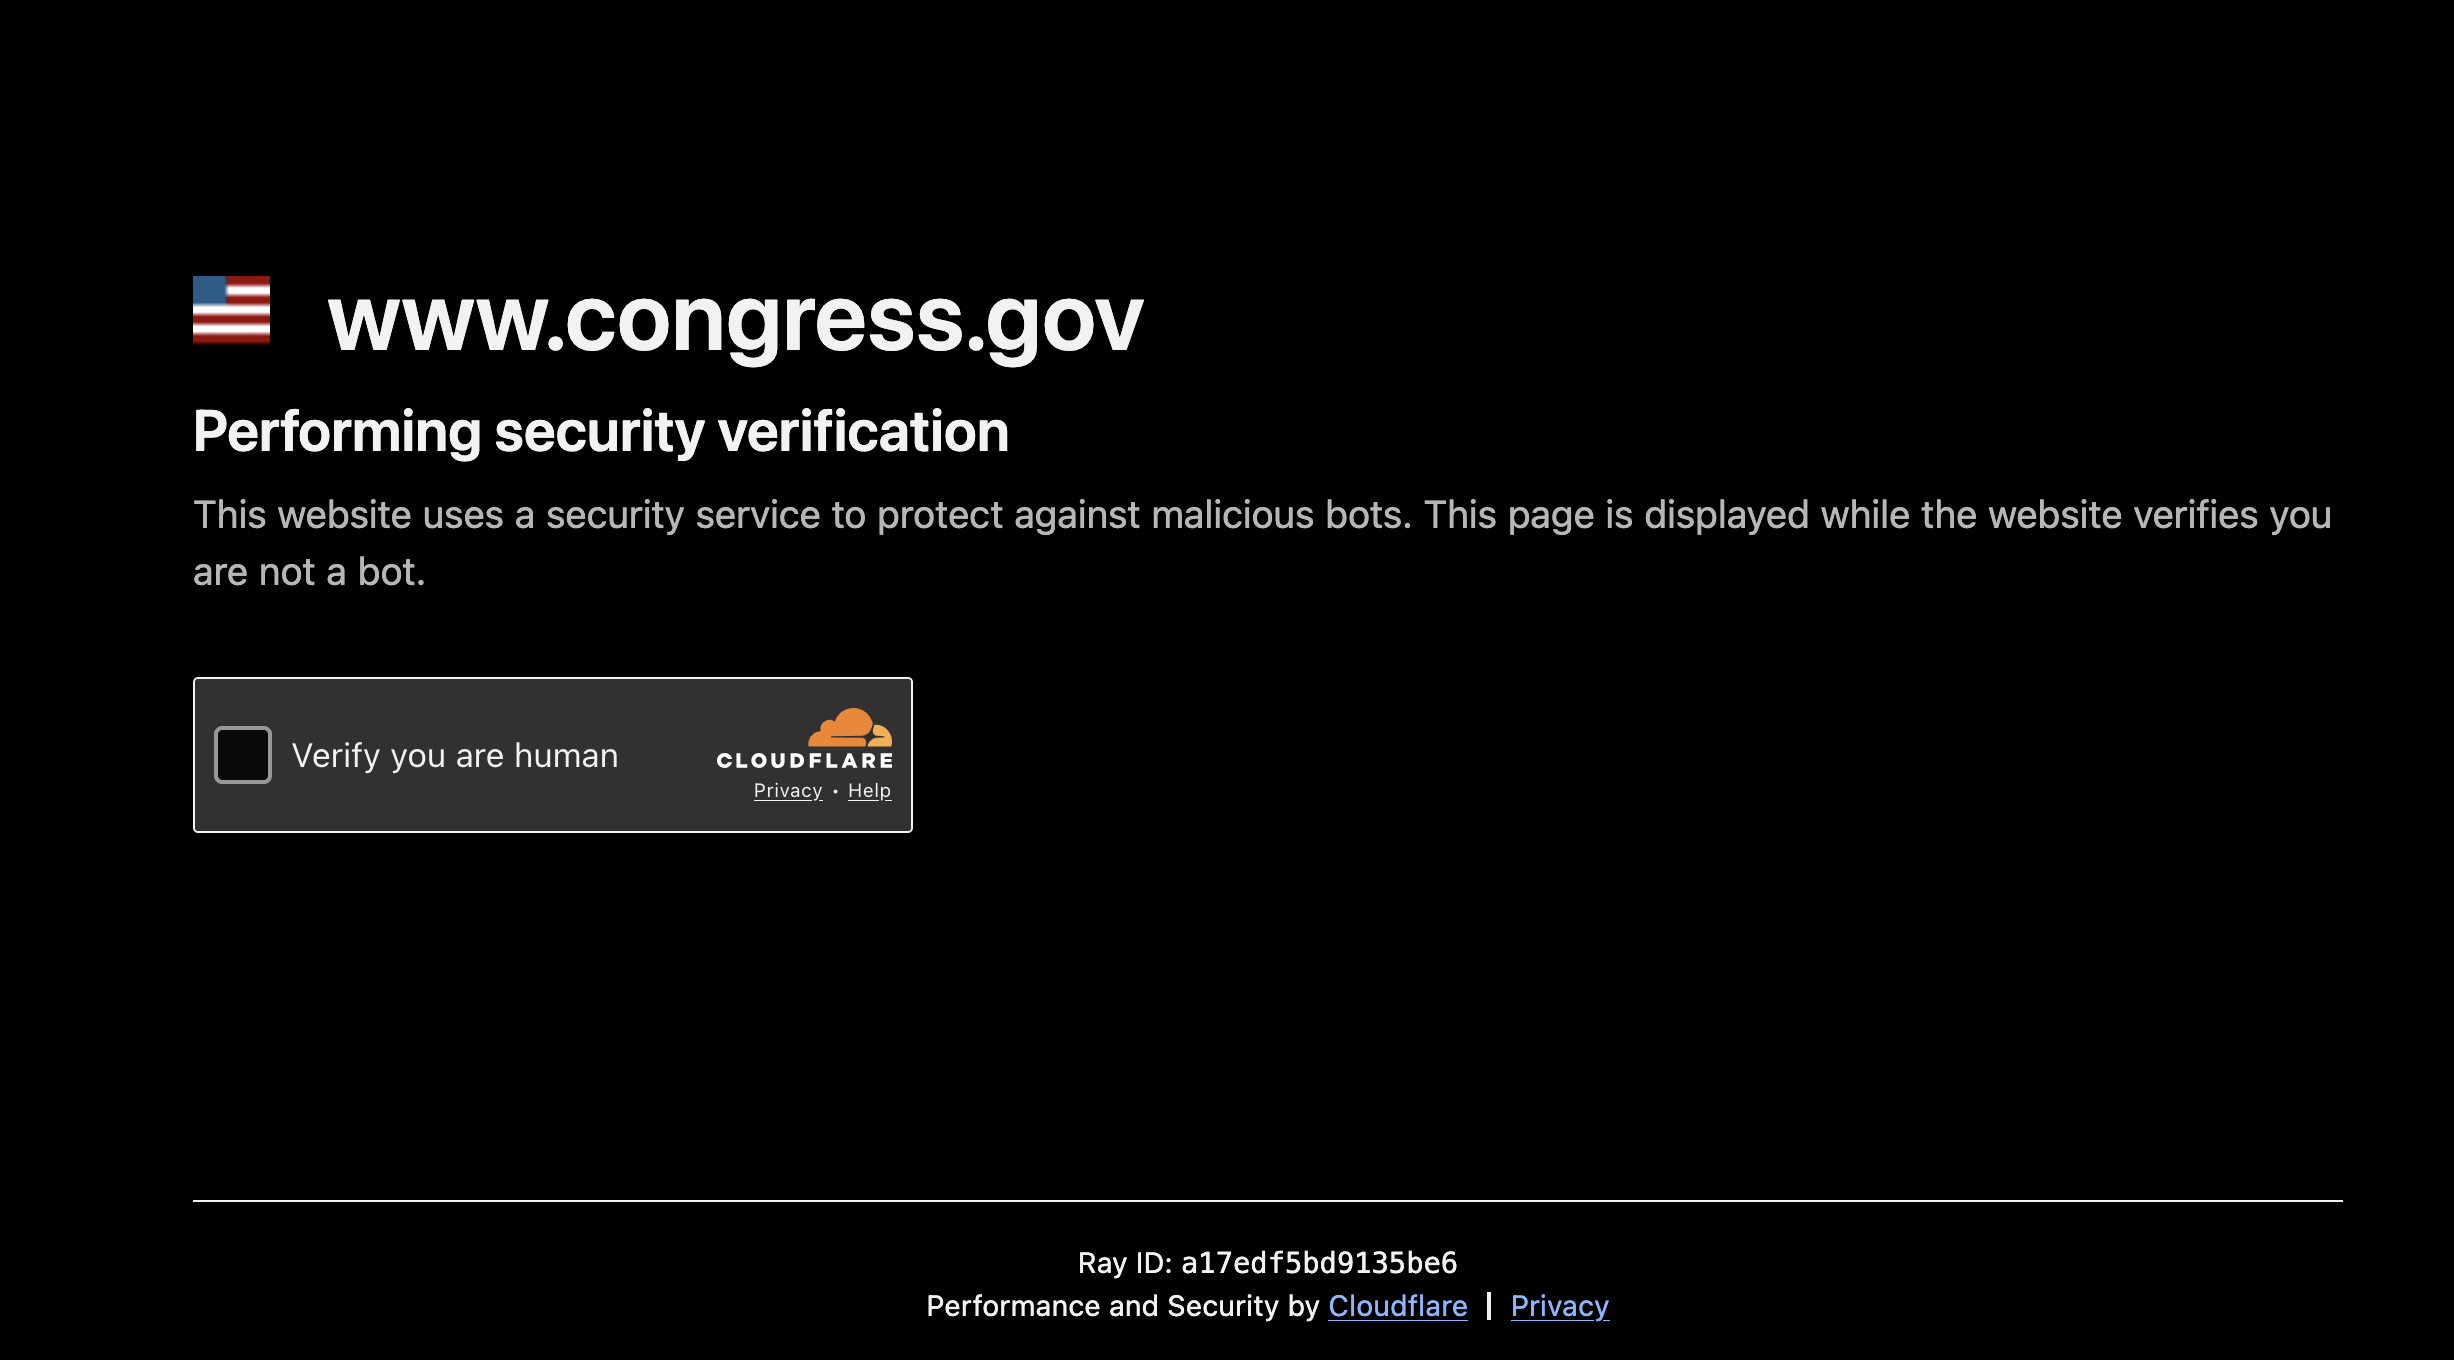
\includegraphics[width=.9\linewidth]{./images/verify.png}
\end{center}

\subsubsection{bypassing blockers: ghost browsers}
\label{sec:orgf6f8e2c}
While these kinds of blockers are more advanced, there are ways of
overcoming them. One method involves using a virtual or "ghost"
browser through python libraries like \texttt{seleniumbase}.

Instead of sending an HTTP request via a python script, \texttt{seleniumbase}
routes the request through an actual web browser, one that is operated
remotely by the python script. When the program is running, a browser
window will open seemingly on its own. Depending on what content the
user wants to scrape, it can then scroll, click on links, or fill in
forms without the input of the user's mouse.

\begin{verbatim}
from seleniumbase import SB

with SB(uc=True, test=True, locale="en") as sb:
    url = "https://www.congress.gov/search?q=%7B%22congress%22%3A%5B%22119%22%5D%2C%22source%22%3A%22all%22%2C%22search%22%3A%22gender%22%7D"
    sb.activate_cdp_mode(url)
    sb.sleep(2)
    sb.solve_captcha()
\end{verbatim}

Because the program is using the actual browser window, it is able to
trick the server into thinking it is a real, not automated, user. By
waiting on the landing page for a few seconds, or even by clicking the
checkbox, as indicated in the function \texttt{solve\_captcha()} above, the
JavaScript that triggers the "Security Verification" could thus
circumvented. With the checkpoint passed, the page loads normally.
Meanwhile, the HTML data is sent to the python program running the
request.

\subsubsection{bypassing blockers: xhr}
\label{sec:org3e73e27}
Besides HTML, there are other data streams, ones that load onto a web
page after the HTML has loaded. Opposed to the \emph{static} data of the
HTML, which loads once and never changes, this kind of data is called
\emph{dynamic} data, and it loads continuously.

Dynamic data cannot be accessed by making a request to the page URL.
Rather, the request must be made to another URL, which is encoded in
the page scripts, which one can access in the "Network" tab in the
browser developer tools.

The XHR, or XML HTTP Request can be used to gather search results,
like the one pictured below. This request, which collects search
results of the keyword "gender" from \texttt{foxnews.com}, gets the data from
a server \texttt{moxie.foxnews.com}, where \emph{Fox News} stores its database of
article information.

\begin{verbatim}
headers = {
    'User-Agent': 'Mozilla/5.0 (Macintosh; Intel Mac OS X 10.15; rv:155.0) Gecko/20100101 Firefox/155.0',
    'Accept': '*/*',
    'Accept-Language': 'en-US,en;q=0.9',
    'Referer': 'https://www.foxnews.com/',
    'Origin': 'https://www.foxnews.com',
    'Connection': 'keep-alive',
    'Sec-Fetch-Dest': 'empty',
    'Sec-Fetch-Mode': 'cors',
    'Sec-Fetch-Site': 'same-site',
}

params = {
    'q': 'gender',
    'fields': 'web',
}

response = requests.get('https://moxie.foxnews.com/search/aggregate/web', params=params, headers=headers)

\end{verbatim}

If a ghost browser mimicks the user, then the XHR request thus mimicks
a web page itself, feigning a request encoded in the page's JavaScript
that would automatically load elements, like search results. 

\subsubsection{bypassing blockers: manipulating the URL}
\label{sec:org988fd29}
\begin{itemize}
\item hacking the URL
\end{itemize}

When dealing with a single website, there is always a work around.


Some pages on a website may block bots, while others do not. For
example, the homepage and search results on \texttt{congress.gov} blocks all
bots, unless the page is accessed through a ghost browser. But even
without a ghost browser, some pages on the \texttt{congress.gov} server can
be scraped, if one knows how to access them.

For example, the full text of congressional bills, which are not
available through the officiall \texttt{congress.gov API},\footnote{Congress.gov API. \url{https://api.congress.gov/\#/}} may be
accessed by reverse engineering the bill URL. The bill URL for
H.R.1927, the "End Taxpayer Funding of Gender Experimentation Act of
2021," proposed by the 117th Congress (2021-2022) can be accessed
at the address below.

\begin{verbatim}
https://www.congress.gov/bill/117th-congress/house-bill/1927
\end{verbatim}

While the full text of this bill (which is under the "text" tab of the
page) cannot be accessed without a ghost browser, it is also stored in
another page on \texttt{congress.gov}.

\begin{verbatim}
https://www.congress.gov/117/bills/hr1927/BILLS-117hr1927ih.htm
\end{verbatim}

The path of the URL is \texttt{/117/bills/hr1927/BILLS-117hr1927ih.html}, in
constrast to the one above, which is
\texttt{/bill/117th-congress/house-bill/1927}. This \texttt{/117} path, unlike the
\texttt{/bill} one, can be scraped using traditional means.

\begin{verbatim}
r = requests.get("https://www.congress.gov/117/bills/hr1927/BILLS-117hr1927ih.htm")
\end{verbatim}

The contents of the request contain the following text, showing the
header of the bill.

\begin{verbatim}
<html><body><pre>
[Congressional Bills 117th Congress]
[From the U.S. Government Publishing Office]
[H.R. 1927 Introduced in House (IH)]

&lt;DOC&gt;






117th CONGRESS
  1st Session
                                H. R. 1927

To prohibit taxpayer-funded gender reassignment medical interventions, 
                        and for other purposes.
\end{verbatim}

This URL has valuable information that would enable one to scrape data
from more bills. With access to another URL for comparison, the a
formula for crafting more URLs could be reverse engineered.

For example, a URL for a different bill, H.R. 8731, "Protect
Children's Innocence Act," also from the 117th congress (2021-2022)
has a similar path to the former bill. Looking at both URLs side by
side displays a pattern in the path's logic.

\begin{verbatim}
https://www.congress.gov/117/bills/hr8731/BILLS-117hr8731ih.htm
https://www.congress.gov/117/bills/hr1927/BILLS-117hr1927ih.htm  
\end{verbatim}

The differences between the two URLs reveals that the bill number,
\texttt{8731} and \texttt{1927} is the only element that changes. With that
knowledge, and with a list of relevant bill numbers (either downloaded
from \texttt{congress.gov} search results or via the API), one can reverse
engineer many---hundreds, in this case---of URLs for scraping. 

\begin{verbatim}
https://www.congress.gov/117/bills/hr1927/BILLS-117hr1927ih.htm
https://www.congress.gov/117/bills/hr8731/BILLS-117hr8731ih.htm
https://www.congress.gov/117/bills/hr5/BILLS-117hr5ih.htm
https://www.congress.gov/117/bills/hr7684/BILLS-117hr7684ih.htm
https://www.congress.gov/117/bills/hr1475/BILLS-117hr1475ih.htm
https://www.congress.gov/117/bills/hr8170/BILLS-117hr8170ih.htm
https://www.congress.gov/117/bills/hr2695/BILLS-117hr2695ih.htm
https://www.congress.gov/117/bills/hr9497/BILLS-117hr9497ih.htm
https://www.congress.gov/117/bills/hr4176/BILLS-117hr4176ih.htm
https://www.congress.gov/117/bills/hr5744/BILLS-117hr5744ih.htm
\end{verbatim}

Below is a function that passes a list of bill numbers into an
algorithm that plugs the number into the URL and scrapes it. The
resulting dataset contains the text for 688 individual bills.

\begin{verbatim}
def scrape_bill_text(bill_numbers):
  bills_text = []
  for number in bill_numbers:
      url = (f''https://www.congress.gov/117/bills/hr{number}/BILLS-117hr{number}ih.htm)
      response = requests.get(url)
      content = response.content
      bills_text.append(content)
  return bills_text
\end{verbatim}

\subsubsection{web crawling: heritage.org}
\label{sec:org522e6cf}
There is another thing: Web crawling.

The automation of scraping multiple pages is called "web crawling."
Traditionally, web crawling is an accretative procedure that involves
scraping a page, gathing the links for that page, and scraping those
pages.

For example, the following web crawler scrapes the search results from
the \texttt{Heritage.org/gender} topic page. The crawler has two functions:
\texttt{parse()}, which scrapes search results, and \texttt{parse\_article()}, which
scrapes article content linked from the search results.

\begin{verbatim}
def parse(self, response):
    article_page_links = response.css("div.result-card__info-wrapper a::attr('href')")
    yield from response.follow_all(article_page_links, self.parse_article)

    # Go to the next page of results
    next_page = response.css('li.pager__item a::attr("href")').get()
    if next_page is not None:
        yield response.follow(next_page, self.parse)
\end{verbatim}
In this function, two important actions are indicated. First, the
\texttt{yield} statement contains another function, \texttt{follow\_all()}, which
first grabs all of the links embedded on that page. Then,
\texttt{follow\_all()} triggers another function, \texttt{parse\_article()}, which
grabs the article text from the linked page. The second important
action is what happens next, which is pagination. The \texttt{parse()}
function will then grab the link for the next page of results, grab
all the result information from that page, and trigger the
\texttt{pare\_article()} function again.

The process then repeats itself, over and over again, until all pages
of results have been scraped. Crawling is thus a recursive process.

\subsection{{\bfseries\sffamily TO\_DRAFT} close reading: heritage foundation}
\label{sec:orge3bc024}
\subsubsection{scaling small}
\label{sec:orgd173f89}
It seems that there is a corruption that is inherent to scale, a
problem first pointed out in Bender et al's titular question, "Can
Language Models be too Big?". As Samual A. Moore writes, “Scalability
banishes meaningful diversity, that is, diversity that might change
things" (Samuel A. Moore, \emph{Publishing Beyond the Market} 147).

Like with the Zyte report, there is a cycle here in which increasing
data and AI technology feed each other. This cycle manifests in real
circular relationships between companies, where AI companies who have
the technology must work with cloud companies who have the necessary
servers and GPUs to handle higher compute. The vast majority of the
capital raised by these AI companies are paid to the cloud providers,
who in turn are responsible for majority of the investment into the AI
companies. As the authors point out, “These circular investment deals
can blur the boundary between 'investment' and 'acquisition'".
(Varoquaux et al 8).
\subsection{{\bfseries\sffamily TO\_DRAFT} conclusion: shame, sedgwick, contagion}
\label{sec:org2acdad1}
\subsubsection{shame as contagion}
\label{sec:orgf1d69a3}
Shame thus moves outward, creating a nexus for interpersonal relation.
Sedgwick links shame to contagion:
\begin{quote}
“Shame—-living, as it does, on and in the muscles and capillaries of
the face—-seems to be uniquely contagious from one person to another.
And the contagiousness of shame is only facilitated by its anamorphic,
protean susceptibility to new expressive grammars" (\emph{Touching Feeling}
63).

“not a discrete intrapsychic structure, but a kind of free radical
that (in different people and different cultures) attaches to and
permanently intensifies or alters the meaning of—-of almost anything:
a zone of the body, a sensory system, a prohibited or indeed a
permitted behavior, another affect such as anger or arousal, a named
identity, a script for interpreting other people’s behavior toward
oneself” (\emph{Touching Feeling} 62)
\end{quote}
In the orbit of queerness, where negative experiences are identity
forming, Sedgwick looks at shame as a positive force.

\begin{quote}
Shame interests me politically, then, because it generates and
legitimates the place of identity--the question of identity\ldots{} without
giving that identity space the standing of an essence. It constitutes
the as-to-be-constituted, which is also to say, as already there for
the (necessary, productive) misconstrual and misrecognition.
(\emph{Touching Feeling} 63)
\end{quote}

\subsubsection{Sedgwick's critique of Butler}
\label{sec:orgbfa014f}
In the influential final pages of Gender Trouble, for example,
Butler
offers a programmatic argument in favor of demystification as
"the normative
focus for gay and lesbian practice,"'" with such
claims as that "drag
implicitly reveals the imitative structure of
gender itself" (137); "we see
sex and gender denaturalizedb y means
of a performance" (138);" gender
parody revealst hat the original
identity \ldots{} is an imitation" (138);" gender
performance will enact
and reveal the performativity of gender itself"
(139); "parodic
repetition \ldots{} exposes the phantasmatic effect of abiding
identity"
(141); "the parodic repetition of gender exposes \ldots{} the illusion
of
gender identity" (146); and "hyperbolic exhibitions of 'the natural'
\ldots{}
reveal its fundamentally phantasmatic status" (147) as well as
"exposing
its fundamental unnaturalness" (149; all emphases added).
(\emph{Novel Gazing} 17). 
\end{document}
